\documentclass[t]{beamer}
\usetheme{Copenhagen}
\usepackage{amsmath, tikz, bm, pgfplots,cancel}
\pgfplotsset{compat=newest}
\pgfplotsset{every tick label/.append style={font=\scriptsize}}
\setbeamertemplate{headline}{} % remove toc from headers
\beamertemplatenavigationsymbolsempty
\everymath{\displaystyle}
% \usepackage[utf8]{inputenc}

\title{Limits and Algebra}
\author{}
\date{}

\AtBeginSection[]
{
  \begin{frame}
    \frametitle{Objectives}
    \tableofcontents[currentsection]
  \end{frame}
}

\begin{document}

\begin{frame}{}
    \maketitle
\end{frame}




\begin{frame}{Intro}
The graphs of $f(x) = \frac{x^2-6x-7}{x-7}$ and $g(x)=x+1$ are \underline{not the same}.	\newline\\	\pause
\begin{tabular}{p{0.5\textwidth}p{0.5\textwidth}}
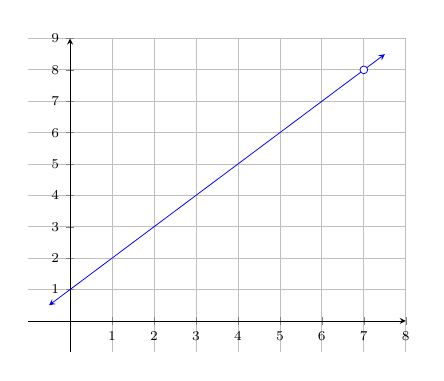
\begin{tikzpicture}[scale=0.7]
\begin{axis}[
	xmin = -1, xmax = 8,
	ymin = -1, ymax = 9,
	axis lines = middle,
	grid,
	xtick = {1,2,...,8},
	ytick = {1,2,...,9}
]
\addplot [<->, >=stealth, domain=-0.5:7.5, color=blue]{x+1};
\addplot [mark = *, color=blue, fill=white] coordinates {(7,8)};
\end{axis}
\end{tikzpicture}
&
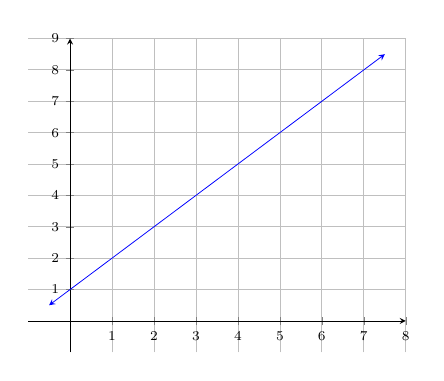
\begin{tikzpicture}[scale=0.7]
\begin{axis}[
	xmin = -1, xmax = 8,
	ymin = -1, ymax = 9,
	axis lines = middle,
	grid,
	xtick = {1,2,...,8},
	ytick = {1,2,...,9}
]
\addplot [<->, >=stealth, domain=-0.5:7.5, color=blue]{x+1};
\end{axis}
\end{tikzpicture}	\\[8pt]
$f(x) = \frac{x^2-6x-7}{x-7}$	&	$g(x)=x+1$	\\
\end{tabular}
\end{frame}

\section{Find Limits via Factoring}

\begin{frame}{Algebraic Limits}
	Some limits that can't be evaluated directly can be evaluated after \alert{cancelling out common factors}.	\newline\\	\pause

	This is called \alert{removable discontinuity}.
\end{frame}

\begin{frame}{Example 1}
	(a) \quad Evaluate $\lim_{x \to -3}\frac{x^2+4x+3}{x+3}$	\newline\\
	\begin{align*}
	\onslide<2->{\lim_{x\to -3} \frac{x^2+4x+3}{x+3} &= \lim_{x \to -3}\frac{(x+3)(x+1)}{x+3}} \\[8pt]
	\onslide<3->{&= \lim_{x\to -3}\frac{\cancel{(x+3)}(x+1)}{\cancel{(x+3)}} } \\[8pt]
	\onslide<4->{&= \lim_{x\to -3} (x+1)} \\[8pt]
	\onslide<5->{&= -3 + 1 } \\[8pt]
	\onslide<6->{&= -2}
	\end{align*}
\end{frame}


\begin{frame}{Example 1}
	(b) \quad Evaluate $\lim_{x\to -2} \frac{x+2}{x^2+7x+10}$	\newline\\
	\begin{align*}
	\onslide<2->{\lim_{x\to -2} \, \frac{x+2}{x^2+7x+10} &= \lim_{x\to -2} \frac{x+2}{(x+2)(x+5)}} \\[8pt]
	\onslide<3->{&= \lim_{x\to -2} \frac{\cancel{x+2}}{\cancel{(x+2)}(x+5)}} \\[8pt]
	\onslide<4->{&= \lim_{x\to -2} \frac{1}{x+5}} \\[8pt]
	\onslide<5->{&= \frac{1}{-2+5}} \\[8pt]
	\onslide<6->{&= \frac{1}{3}}
	\end{align*}
\end{frame}

\section{Limits with Complex Fractions}

\begin{frame}{Complex Fractions}
Simplify the complex fraction by multiplying every term by the \alert{least common tiny denominator}.
\end{frame}

\begin{frame}{Example 2}
Evaluate each.	\newline\\
(a) \quad $\lim_{x\to -5} \left(\frac{\frac{1}{x} + \frac{1}{5}}{x+5}\right)$	\newline\\
\begin{align*}
	\onslide<2->{\lim_{x\to -5} \left(\frac{\frac{1}{x} + \frac{1}{5}}{x+5}\right) &= \lim_{x\to -5} \left(\frac{\frac{1}{x} + \frac{1}{5}}{x+5}\right) \left(\frac{5x}{5x}\right)}	\\[8pt]
	\onslide<3->{&= \lim_{x\to -5} \frac{5+x}{5x(x+5)}} \\
\end{align*}
\end{frame}

\begin{frame}{Example 2}
\begin{align*}
	&= \lim_{x\to -5} \frac{\cancel{5+x}}{5x\cancel{(x+5)}} \\[8pt]
	\onslide<2->{&= \lim_{x\to -5} \frac{1}{5x}} \\[8pt]
	\onslide<3->{&= \frac{1}{5(-5)}} \\[8pt]
	\onslide<4->{&= -\frac{1}{25}} 
\end{align*}
\end{frame}

\begin{frame}{Example 2}
(b) \quad $\lim_{x\to 3} \left(\frac{\frac{1}{3}-\frac{1}{x}}{3-x}\right)$	\newline\\
\begin{align*}
	\onslide<2->{\lim_{x\to 3} \left(\frac{\frac{1}{3}-\frac{1}{x}}{3-x}\right) &= \lim_{x\to 3} \left(\frac{\frac{1}{3}-\frac{1}{x}}{3-x}\right) \left(\frac{3x}{3x}\right)}	\\[10pt]
	\onslide<3->{&= \lim_{x\to 3} \frac{x-3}{3x(3-x)}} \\
\end{align*}
\end{frame}

\begin{frame}{Example 2}
\begin{align*}
	&= \lim_{x\to 3} \frac{\cancel{x-3}}{3x\cancel{(3-x)}} \\[10pt]
	\onslide<2->{&= \lim_{x\to 3} \frac{-1}{3x}} \\[10pt]
	\onslide<3->{&= \frac{-1}{3(3)}} \\[10pt]
	\onslide<4->{&= \frac{-1}{9}}
\end{align*}
\end{frame}

\section{Limits with Radicals}

\begin{frame}{Radicals}
When working with radicals, multiply by the \alert{conjugate}.	\newline\\

\begin{center}
\begin{tabular}{cc}
\textbf{Expression} & \textbf{Conjugate} \\[6pt]
$a + \sqrt{b}$ & $a - \sqrt{b}$ \\[6pt]
$a - \sqrt{b}$ & $a + \sqrt{b}$ \\
\end{tabular}
\end{center}
\end{frame}

\begin{frame}{Example 3}
(a) \quad $\lim_{x\to 0} \left(\frac{\sqrt{25-x}-5}{x}\right)$	
\begin{align*}
\onslide<2->{\lim_{x\to 0} \left(\frac{\sqrt{25-x}-5}{x}\right) &= \lim_{x\to 0} \left(\frac{\sqrt{25-x}-5}{x}\right)\left(\frac{\sqrt{25-x}+5}{\sqrt{25-x}+5}\right)}	\\[8pt]
\onslide<3->{&= \lim_{x\to 0} \frac{25-x-25}{x\left(\sqrt{25-x}+5\right)}}	\\[8pt]
\onslide<4->{&= \lim_{x\to 0} \frac{-x}{x\left(\sqrt{25-x}+5\right)}}	\\
\end{align*}
\end{frame}

\begin{frame}{Example 3}
\begin{align*}
&= \lim_{x\to 0} \frac{-1}{\sqrt{25-x}+5}	\\[8pt]
\onslide<2->{&= \frac{-1}{\sqrt{25-0}+5}}	\\[8pt]
\onslide<3->{&= \frac{-1}{10}}
\end{align*}
\end{frame}

\begin{frame}{Example 3}
(b) \quad $\lim_{h\to 0} \left(\frac{\sqrt{16+h}-4}{h}\right)$
\begin{align*}
\onslide<2->{\lim_{h\to 0} \left(\frac{\sqrt{16+h}-4}{h}\right) &= \lim_{h\to 0} \left(\frac{\sqrt{16+h}-4}{h}\right)\left(\frac{\sqrt{16+h}+4}{\sqrt{16+h}+4}\right)}	\\[8pt]
\onslide<3->{&= \lim_{h\to 0} \frac{16+h-16}{h\left(\sqrt{16+h}+4\right)}} \\[8pt]
\onslide<4->{&= \lim_{h\to 0} \frac{h}{h\left(\sqrt{16+h}+4\right)}}	\\
\end{align*}
\end{frame}

\begin{frame}{Example 3}
\begin{align*}
&= \lim_{h\to 0} \frac{1}{\sqrt{16+h}+4}	\\[8pt]
\onslide<2->{&= \frac{1}{\sqrt{16+0}+4}} \\[8pt]
\onslide<3->{&= \frac{1}{8}}
\end{align*}
\end{frame}

\begin{frame}{Example 3}
(c) $\lim_{x\to 4} \frac{4-x}{\sqrt{x}-2}$
\begin{align*}
\onslide<2->{\lim_{x\to 4} \frac{4-x}{\sqrt{x}-2} &= \lim_{x\to 4} \frac{4-x}{\sqrt{x}-2} \left(\frac{\sqrt{x}+2}{\sqrt{x}+2}\right)} \\[8pt]
\onslide<3->{&= \lim_{x\to 4} \frac{(4-x)(\sqrt{x}+2)}{x-4}} \\[8pt]
\onslide<4->{&= \lim_{x\to 4} -1(\sqrt{x}+2)}	\\[8pt]
\onslide<5->{&= -1(\sqrt{4}+2)} \\[8pt]
\onslide<6->{&= -1(2+2) = -4}
\end{align*}
\end{frame}

\begin{frame}{Example 3}
(d) \quad $\lim_{x\to 3} \frac{x-3}{\sqrt{x}-\sqrt{3}}$
\begin{align*}
\onslide<2->{\lim_{x\to 3} \frac{x-3}{\sqrt{x}-\sqrt{3}} &= \lim_{x\to 3} \frac{x-3}{\sqrt{x}-\sqrt{3}}\left(\frac{\sqrt{x}+\sqrt{3}}{\sqrt{x}+\sqrt{3}}\right)}	\\[8pt]
\onslide<3->{&= \lim_{x\to 3} \frac{(x-3)(\sqrt{x}+\sqrt{3})}{x-3}} \\[8pt]
\onslide<4->{&= \lim_{x\to 3} (\sqrt{x}+\sqrt{3})} \\[8pt]
\onslide<5->{&= \sqrt{3}+\sqrt{3}} \\[8pt]
\onslide<6->{&= 2\sqrt{3}}
\end{align*}
\end{frame}

\section{Limits with Absolute Value}

\begin{frame}{Limits and Absolute Value}
With absolute value, it might be better to use a table or a graph to find the limit.	\newline\\ \pause

Also, look at the left-hand and right-hand limits.
\end{frame}

\begin{frame}{Example 4}
Find the limit for each.	\newline\\
(a) \quad $\lim_{x\to 7} \frac{|x-7|}{x-7}$	\newline\\

\begin{minipage}{0.6\textwidth}
\onslide<2->{
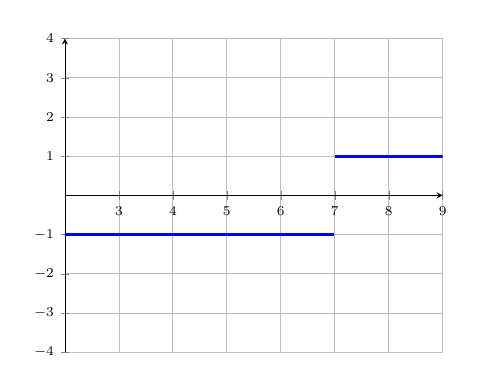
\begin{tikzpicture}[scale=0.7]
\begin{axis}[
axis lines = middle,
grid,
xmin = 2, xmax = 9,
ymin = -4, ymax = 4,
xtick = {3,...,9},
ytick = {-4,-3,...,4}
]
\addplot[color=blue, domain=1:6.99, ultra thick] {abs(x-7)/(x-7)};
\addplot[color=blue, domain=7.01:9, ultra thick] {abs(x-7)/(x-7)};
\end{axis}
\end{tikzpicture}}
\end{minipage}
\hspace{0.25cm}
\begin{minipage}{0.3\textwidth}
\begin{align*}
\onslide<3->{& \lim_{x\to 7^-} \frac{|x-7|}{x-7}} 
\onslide<4->{= -1} \\[10pt]
\onslide<5->{& \lim_{x\to 7^+} \frac{|x-7|}{x-7}} 
\onslide<6->{= 1} \\[10pt]
\onslide<7->{& \text{\alert{Does Not Exist}}}
\end{align*}
\end{minipage}
\end{frame}

\begin{frame}{Example 4}
(b) \quad $\lim_{x \to 6^+} \frac{6-x}{|x-6|}$	\newline\\
\begin{minipage}{0.6\textwidth}
\onslide<2->{
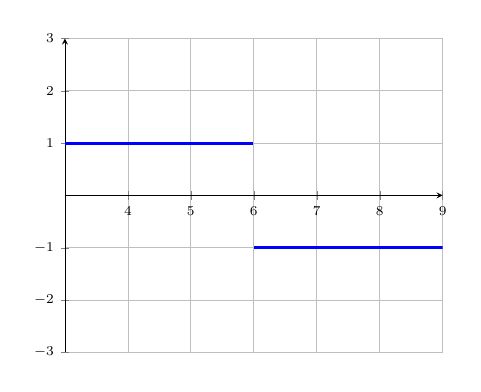
\begin{tikzpicture}[scale=0.7]
\begin{axis}[
	axis lines = middle,
	grid,
	xmin = 3, xmax = 9,
	ymin = -3, ymax = 3,
	xtick = {3,4,...,9},
	ytick = {-3,-2,...,3}
]
	\addplot[color=blue, ultra thick, domain=6.01:9] {(6-x)/abs(x-6)};
	\addplot[color=blue, ultra thick, domain=3:5.99] {(6-x)/abs(x-6)};
\end{axis}
\end{tikzpicture}}
\end{minipage}
\hspace{0.25cm}
\begin{minipage}{0.3\textwidth}
\begin{align*}
\onslide<3->{& \lim_{x \to 6^+} \frac{6-x}{|x-6|}}
\onslide<4->{&= \alert{-1}} \\
\end{align*}
\end{minipage}
\end{frame}

\end{document}
